The System Usability Scale (SUS) is a ten-question questionnaire, each with a
five-point response scale ranging from Strongly Disagree to Strongly Agree.
These questions are divided into two types:

\begin{enumerate}
  \item Odd-numbered items, considered the positive statements
    (\Cref{fig:statements_results_sus_positive}).
  \item Even-numbered items, considered the negative statements
    (\Cref{fig:statements_results_sus_negative}).
\end{enumerate}

The division of the questions into positive and negative statements provides
valuable insights into the overall usability of the application. Better user
experience and usability mean the questionnaire tends to have higher
evaluations (agreement) on positive statements. Conversely, lower evaluations
(disagreement) are desired on negative statements, indicating fewer usability
issues or challenges. The aim is to achieve higher ratings on the positive
statements and lower ratings on the negative statements, as this indicates a
more favourable user perception of the application's usability.

\begin{figure*}[!htb]
  \centering
  \begin{subfigure}[b]{1\textwidth}
    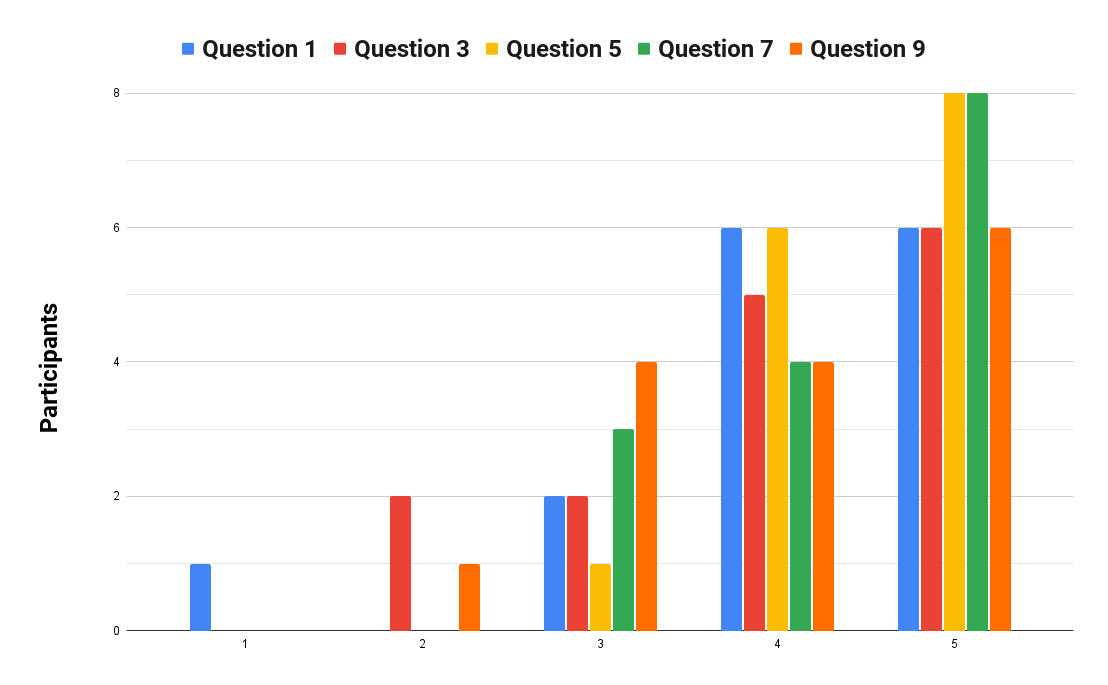
\includegraphics[width=\textwidth]{sus_positive}
    \caption{Positive Statements}
    \label{fig:statements_results_sus_positive}
  \end{subfigure}
  \hfill
  \begin{subfigure}[b]{1\textwidth}
    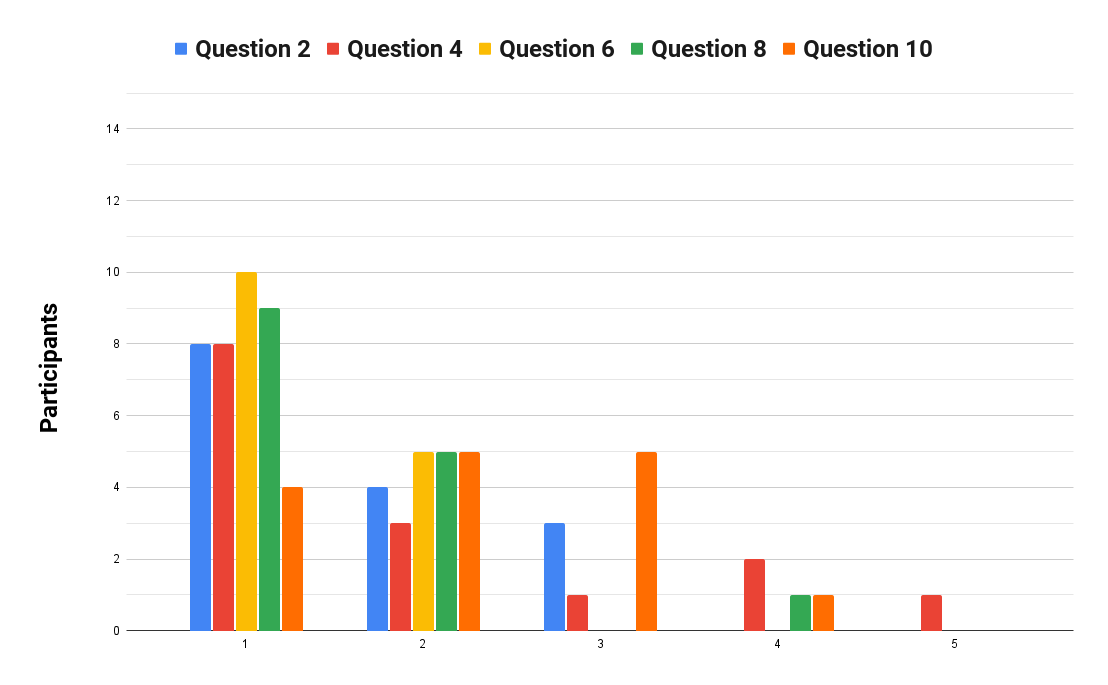
\includegraphics[width=\textwidth]{sus_negative}
    \caption{Negative Statements}
    \label{fig:statements_results_sus_negative}
  \end{subfigure}
  \caption{Statements Results SUS}
  \label{fig:statements_results_sus}
\end{figure*}

By analysing the results of the statements in
\Cref{fig:statements_results_sus}, it becomes evident that most participants
provided higher evaluations for the positive statements. Approximately 79\% of
participants rated these positive statements at level four or higher,
indicating a positive perception of the application's usability, while only a
tiny proportion (7\%) of participants selected level two or lower for the
positive statements.

On the other hand, the negative statements received lower evaluations from the
participants. Around 81\% of participants rated these negative statements at
level two or lower, suggesting a relatively low occurrence of usability issues,
and a minimal percentage (5\%) of participants provided evaluations at level
four or higher for the negative statements.

The average SUS Score for each participant was found to be 80.3 out of 100,
indicating a generally positive perception of the application's usability. The
median SUS Score was calculated to be 85 out of 100, further supporting the
positive evaluation.

The quartiles, representing the distribution of the SUS Scores, are presented
in \Cref{tab:sus_quartiles}. Additionally, a corresponding box plot graphic in
\Cref{fig:sus_box_plot} visualises the distribution of the scores, providing a
visual representation of the SUS Score data.

\begin{table}[!htb] \caption{SUS Quartiles} \label{tab:sus_quartiles}
  \begin{center}
    \begin{tabular}[c]{p{8em}|p{8em}}
      \textbf{Quartile} &
      \textbf{Value} \\
      \hline 0 & 42,5 \\
      \hline 1 & 65.75 \\
      \hline 2 & 85 \\
      \hline 3 & 93.75 \\
      \hline 4 & 97.5 \\
    \end{tabular}
  \end{center}
\end{table}

\begin{figure*}[!htb]
  \centering
  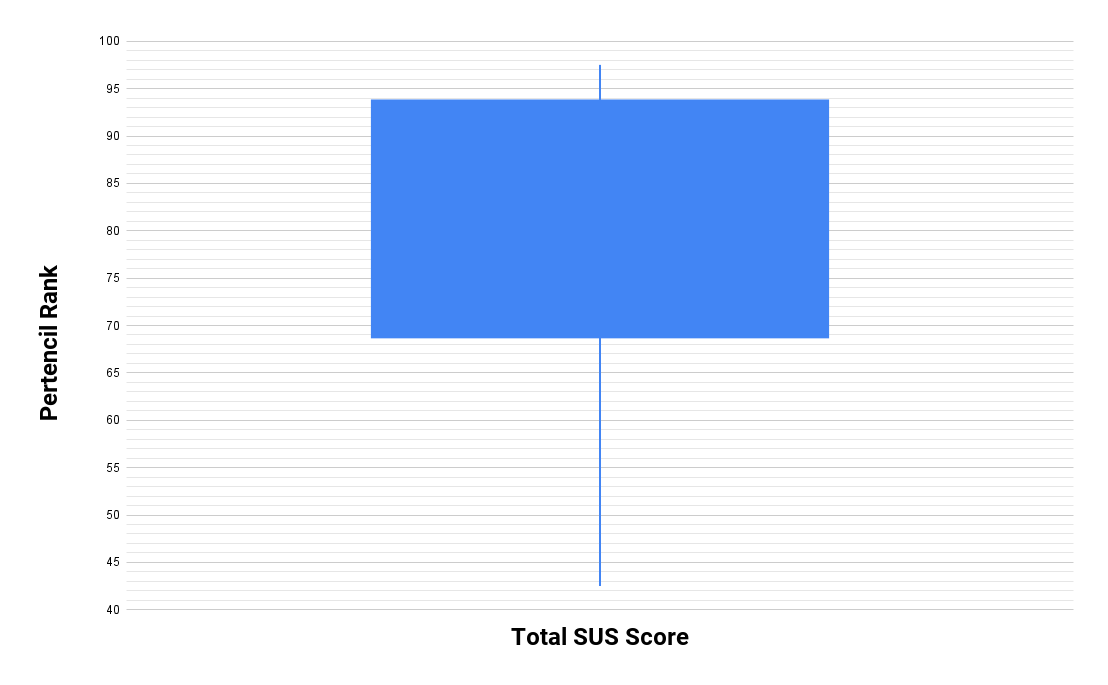
\includegraphics[width=\textwidth]{sus_score_box_plot}
  \caption{SUS Box Plot}
  \label{fig:sus_box_plot}
\end{figure*}

Participants with experience in microservices, those who have worked with
microservices and have experience in decomposing monoliths into microservices,
have higher evaluations in positive statements and lower evaluations in
negative statements, as evidenced in
\Cref{fig:statements_results_sus_positive_exp,fig:statements_results_sus_negative_exp},
respectively.

\begin{figure*}[!htb]
  \centering
  \begin{subfigure}[b]{1\textwidth}
    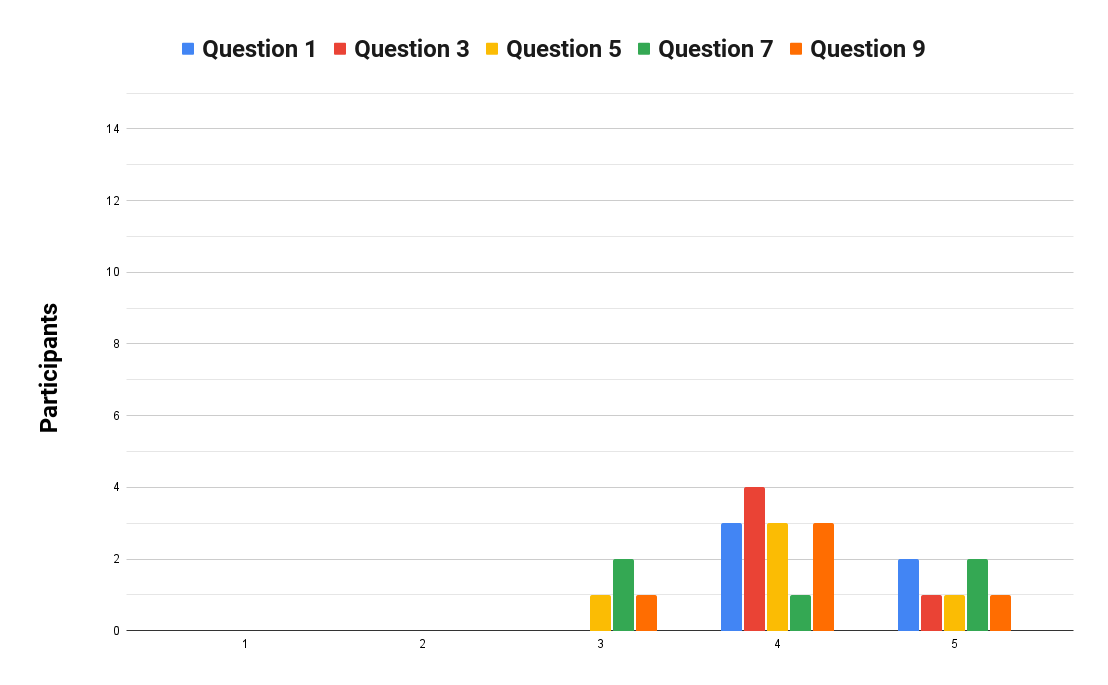
\includegraphics[width=\textwidth]{sus_positive_exp}
    \caption{Positive Statements}
    \label{fig:statements_results_sus_positive_exp}
  \end{subfigure}
  \hfill
  \begin{subfigure}[b]{1\textwidth}
    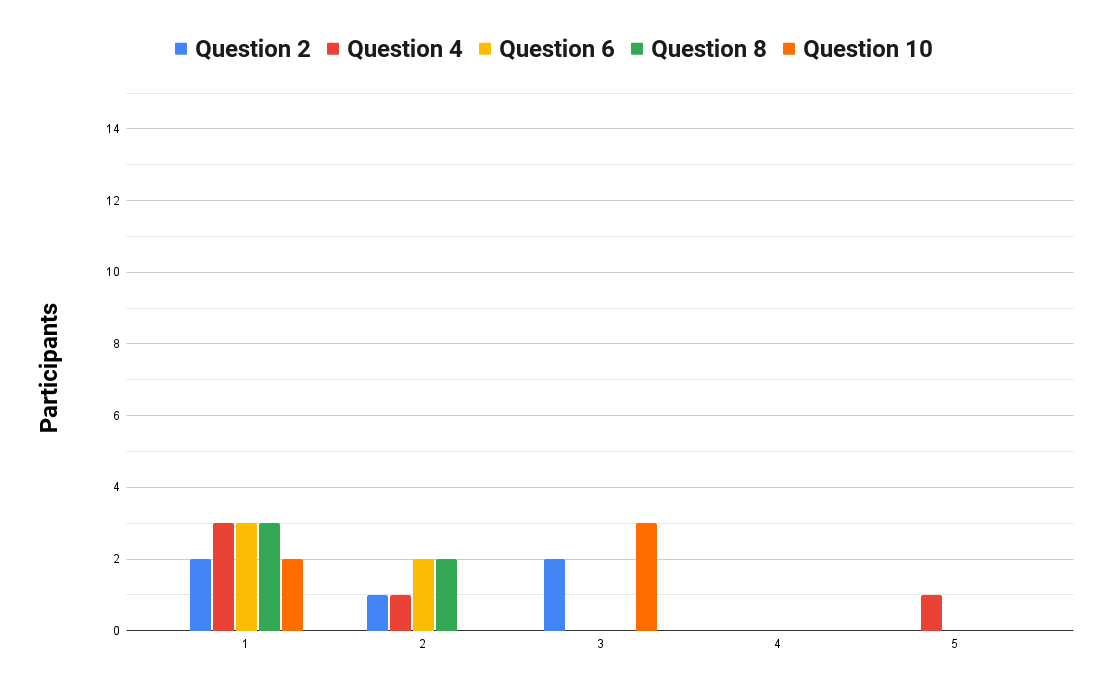
\includegraphics[width=\textwidth]{sus_negative_exp}
    \caption{Negative Statements}
    \label{fig:statements_results_sus_negative_exp}
  \end{subfigure}
  \caption{Experienced Participants Statements Results SUS}
  \label{fig:statements_results_sus_exp}
\end{figure*}
